\documentclass[prl,aps,twocolumn,floatfix,amsmath,amssymb,superscriptaddress,tightenlines]{revtex4}
\usepackage{graphicx}% Include figure files
%\usepackage{amsmath}
\usepackage{amsfonts}
\usepackage{bm}
%\bibliographystyle{prsty}
\begin{document}

\date{\today}
\title{Valence Bond and von Neumann Entanglement Entropy in Heisenberg Ladders}
%\author{Ann Kallin}
%\affiliation{Department of Physics and Astronomy, University of Waterloo, Ontario, N2L 3G1, Canada} 


\begin{abstract}

\end{abstract}
\maketitle

%\newpage

Entanglement has arisen in condensed matter physics as a new paradigm for the study of correlations in a system.  Measurements of entanglement between separate subregions, chiefly using entropic quantities, have one advantage over traditional two-point correlation functions in that they encode the total amount of information shared between two subregions without the possibility of missing ``hidden'' correlations.  Such hidden correlations may occur in some quantum groundstates,  in particular the important example of spin liquid states, where two-point correlation functions decay at large lengthscales.  However, it is well known that a type of topological order may exist in spin liquids, which may be quantified in a ``topological entanglement entropy'', a property of the groundstate wavefunction.  This and other entropic measures are typically discussed in the context of the von Neumann entropy, defined for a bipartitioned region A as
\begin{equation}
S^{\rm VN}_A = - {\rm Tr} \rho_A \ln \rho_A
\end{equation}
where the reduced density matrix $\rho_A = {\rm Tr}_B | \psi \rangle \langle \psi |$ is obtained by tracing out the rest of the system B.

The von Neumann (VN) entanglement entropy (EE) has a well-defined and well-studied set of analytical properties in interacting quantum systems.  In one dimension (1D), exact analytical results are known from conformal field theories (CFT); they show, among other things, that the VN EE between A and B scales according to the boundary.  This so-called {\it area law} is also believed to hold in many groundstates of two dimensional (2D) interacting quantum Hamiltonians, although few exact results are available.  
Of particular importance, the existence of an area law has consequences in the rapidly-advancing field of computational quantum-many body theory: it is believed that if the groundstate of a 2D Hamiltonian obeys an area law, then this groundstate may be represented by a Matrix Product State (MPS).  Such MPS states are the basis for a new promising class of numerical algorithms that promise to push our abilities to study 2D quantum systems with unbiased simulation past the current state of the art quantum Monte Carlo (QMC) technologies, which are hampered by the notorious fermionic sign problem.

\begin{figure}
{
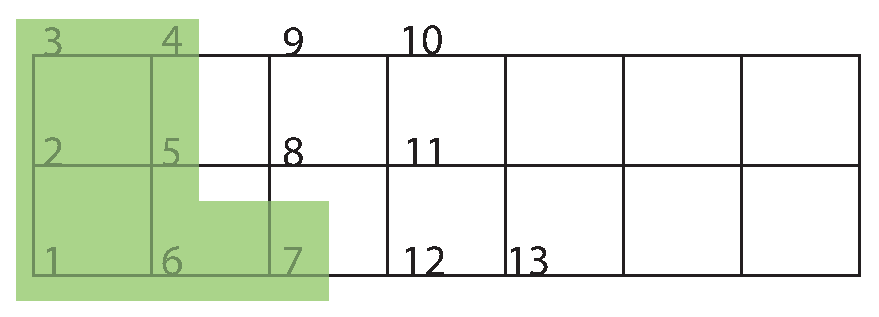
\includegraphics[width=2.4in]{ladder.eps}
\caption{(color online) A three-leg ladder.  The site labels $x$ indicate the order in which DMRG sweeping takes place, which is also the index order by which entanglement entropy is measured.  The blue box labels sites in the region A, with $x=7$.
\label{ladder}}}
\end{figure}

Thus the question of an area law in the groundstates of 2D quantum systems is of utmost important for the development of new simulation techniques.  Paradoxically, it is also a quantity that is difficult to measure in 2D systems, due to the fact that QMC techniques (currently the only scalable method capable of unbiased 2D simulations) do not have direct access to the groundstate wavefunction $\psi$, required to construct the VN EE.  In response to this, several authors \cite{Alet} has recently introduced the concept of {\it valence bond} (VB) entanglement entropy, defined for an SU(2) symmetric spin system as
\begin{equation}
S^{\rm VB}_A = \ln(2) \cdot N_A,
\end{equation}
where $N_A$ is the number of EPR spin singlets ${( |\uparrow \downarrow \rangle - | \downarrow \uparrow \rangle)/\sqrt{2}}$ crossing the boundary between regions A and B.  Unlike the VN EE, the VB EE can be accessed very easily in the valence-bond basis projector QMC method recently proposed by Sandvik.  Although many specific properties of the VB EE can be shown to be different than the VN EE, it is the proposal in Ref. that many quantitative and qualitative features of the VN EE are shared by it.   In particular, measurements of the VB EE in 1D show expected behavior, including area laws,  known in many cases from CFT.  Most striking however is the observation that the VB EE in the case of the Neel groundstate of the isotropic Heisenberg Hamiltonian displays a {\it multiplicative} logarithmic correction to the area law.  If this property were indeed shared by the VN EE, it would have the consequence that the prototypical 2D Neel groundstate is, among other things, not representable by a MPS.

In this paper, we compare the VB EE calculated by valence-bond QMC to the VN EE accessible through large-scale density-matrix renormalization group (DMRG) measurements on the Heisenberg model on multi-leg ladder geometries.    We show...

The spin 1/2 Heisenberg hamiltonian is given by
\begin{equation}
H = J \sum_{\langle i j \rangle} {\mathbf S}_i \cdot {\mathbf S}_j \label{ham}
\end{equation}
where the sum is over nearest-neighbor sites on a ladder with length $L$ and legs $n$.  Many properties of this model on open-boundary ladders with $n$ legs has been exhaustively studied.  Of importance, it is known that a spin gap exists for even-$n$ ladders in the limit of $L\rightarrow \infty$, whereas odd-$n$ ladders behave somewhat more like quasi-1D  systems with spin $n/2$ and, from Haldane's conjecture, are therefore gapless.  

We employ two complementary numerical techniques in our study of EE on ladder geometries, namely the valence-bond basis QMC and DMRG, both of which give {\it unbiased} approximations to the ground state of the Hamiltonian at zero temperature, and results from both of which can be compared directly to one another.  Of interest to us are the two definitions of entanglement entropy; the VN EE is naturally accessible through the DRMG ``sweeping'' algorithm, which converges the groundstate wavefunction of a finite-size system by calculating the reduced density matrix between a ``system'' and ``environment'' (subregions A and B), the size of each of which are systematically grown or reduced in the usual DMRG sweep.  The reduced density matrix $\rho_A$ is calculated at each sweeping step, therefore the VN EE is immediately available for geometries illustrated in Fig.~\ref{ladder}.  In this paper, we label the regions A by the largest lattice site $x$ contained therein.

The valence-bond basis QMC algorithm that we use is the simple single-projector method, with lattice geometries constructed to match those given by the DMRG algorithm.  
***ANN: ENTER DESCRIPTION OF VB QMC HERE***

\begin{figure}
{

\includegraphics[width=3.0in]{fig1.eps}
\caption{(color online) The valence bond and von Neumann entanglement entropies for a 1D Heisenberg chain with 100 sites.
\label{1D}}}
\end{figure}

We consider first the case of a one-dimensional Heisenberg chain, limiting ourselves to a discussion of the system with open boundary conditions (OBC), in order to retain the maximal efficiency of the DMRG, which is known to have poorer convergence properties under periodic boundary conditions (PBC).  For the isotropic OBC chain with Hamiltonian Eq.~\eqref{ham} with some interior point subdividing the region A of length $x$ from the remainder of the system, the von Neumann entropy is known from conformal field theory (CFT) to obey $S^{VN}_A = c/6 \ln(x') + S_1$, where $c=1$ is the central charge, and $x'=L/\pi \sin(\pi x / L)$ is the conformal distance \cite{Cardy}.
In Ref.~\cite{Alet}, VB EE calculated from QMC was compared to this CFT result, and a good fit to a central charge of $c=1$ was found.  In Fig.~XXX we compare this result to the VN EE calculated from the DRMG.  We stress that the QMC and DMRG results are on the same geometry and Hamiltonian, and reproduce the same ground state energies; the remaining figures in the paper can be considered as exact comparisons between the VB and VN EE as calculated with the two methods.
***DISCUSSION***

\bibliography{VB_biblio}


\end{document}
